\iffalse

INSTRUCTIONS: (if this is not lecture1.tex, use the right file name)

  Clip out the ********* INSERT HERE ********* bits below and insert
appropriate TeX code.  Once you are done with your file, run

  ``latex lecture1.tex''

from a UNIX prompt.  If your LaTeX code is clean, the latex will exit
back to a prompt.  Once this is done, run

  ``dvips lecture1.dvi''

which should print your file to the nearest printer.  There will be
residual files called lecture1.log, lecture1.aux, and lecture1.dvi.
All these can be deleted, but do not delete lecture1.tex.
\fi
%
\documentclass[11pt]{article}
\usepackage{amsfonts}
\usepackage{amsmath}
\usepackage{latexsym}
\usepackage{hyperref}
\usepackage{tikz}
\usepackage{listings}

\hypersetup{
    colorlinks=true,
    linkcolor=blue,
    filecolor=magenta,      
    urlcolor=cyan,
}
 
\urlstyle{same}

\setlength{\oddsidemargin}{.25in}
\setlength{\evensidemargin}{.25in}
\setlength{\textwidth}{6in}
\setlength{\topmargin}{-0.4in}
\setlength{\textheight}{8.5in}

\newcommand{\handout}[5]{
   %\renewcommand{\thepage}{#1-\arabic{page}}
   \noindent
   \begin{center}
   \framebox{
      \vbox{
    \hbox to 5.78in { {\bf Data Structures and Algorithms} \hfill #2 }
       \vspace{4mm}
       \hbox to 5.78in { {\Large \hfill #5  \hfill} }
       \vspace{2mm}
       \hbox to 5.78in { {\it #3 \hfill #4} }
      }
   }
   \end{center}
   \vspace*{4mm}
}

\newcommand{\lecture}[3]{\handout{L#1}{#2}{}{}{#1}}

\def\squarebox#1{\hbox to #1{\hfill\vbox to #1{\vfill}}}
\def\qed{\hspace*{\fill}
        \vbox{\hrule\hbox{\vrule\squarebox{.667em}\vrule}\hrule}}
\newenvironment{solution}{\begin{trivlist}\item[]{\bf Solution:}}
                      {\qed \end{trivlist}}
\newenvironment{solsketch}{\begin{trivlist}\item[]{\bf Solution Sketch:}}
                      {\qed \end{trivlist}}
\newenvironment{proof}{\begin{trivlist}\item[]{\bf Proof:}}
                      {\qed \end{trivlist}}

\newtheorem{theorem}{Theorem}
\newtheorem{corollary}[theorem]{Corollary}
\newtheorem{lemma}[theorem]{Lemma}
\newtheorem{observation}[theorem]{Observation}
\newtheorem{remark}[theorem]{Remark}
\newtheorem{proposition}[theorem]{Proposition}
\newtheorem{definition}[theorem]{Definition}
\newtheorem{Assertion}[theorem]{Assertion}
\newtheorem{fact}[theorem]{Fact}
\newtheorem{hypothesis}[theorem]{Hypothesis}
%\newtheorem{observation}[theorem]{Observation}
%\newtheorem{proposition}[theorem]{Proposition}
\newtheorem{claim}[theorem]{Claim}
\newtheorem{assumption}[theorem]{Assumption}

%Put more macros here, as needed.
\newcommand{\al}{\alpha}
\newcommand{\Z}{\mathbb Z}
\newcommand{\jac}[2]{\left(\frac{#1}{#2}\right)}
\newcommand{\set}[1]{\{#1\}}

\def\ppt{{\sf PPT}}
\def\poly{{\sf poly}}
\def\negl{{\sf negl}}
\def\owf{{\sf OWF}}
\def\owp{{\sf OWP}}
\def\tdp{{\sf TDP}}
\def\prg{{\sf PRG}}
\def\prf{{\sf PRF}}

%end of macros
\begin{document}
\fbox{
\vbox{
\begin{flushleft}
Hudson Cho, Ryan Wilson, Jesse Washburn, Colin Shuster, Samhith Patibandla\\  % authors' names
COSC 336 \\  %class
03/11/2025\\  % date
\end{flushleft}
\center{\Large{\textbf{Assignment 4}}}
%\end{mdframed}
} % end vbox
} % end fbox
\vline

\textbf{Instructions.}
\begin{enumerate}
\item Due date and time: As indicated on Blackboard. 
\item This is a team assignment. Work in teams of 3-4 students.  Submit on Blackboard one assignment per team, with the names of all students making the team. 
\item The exercises will not be graded, but you still need to present your best attempt to solve them. If you do not know how to solve an exercise, say it.  This will give me feedback about your understanding of the theoretical concepts.
\item Your programs must be written in Java.

\item Write your programs neatly - imagine yourself grading your program and see if it is easy to read and understand. 

Comment your programs reasonably: there is no need to comment lines like "i++" but do include brief comments describing the main purpose of a specific block of lines.
\item  You will submit on \textbf{Blackboard} 32 files.  

The \textbf{1-st file} is a pdf file (produced ideally with latex and Overleaf) and it will contain the following:
\begin{enumerate}
\item The solution to the Exercises (see the remark above).
\item   A short description of your algorithm for the Programming Task, where you explain the dynamic programing approach. Focus on how you have modified MERGE.
\item   A table with the results your program gives  for the data sets indicated for the programming task. 
\item   The java code (so that the grader can make observations) of the  program.
\end{enumerate}


The \textbf{2-nd file} is the .java file containing the java source code for Programming Task.

\end{enumerate}
\newpage

\if01
\textbf{Instructions.}
\begin{enumerate}
\item Due date and  time: As announced on Blackboard.
\item This is a team assignment. Work in teams as in the previous assignments.  Submit one assignment per team, with the names of all students making the team.
\item Your programs must be written in Java.
\item Write your programs neatly - imagine yourself grading your program and see if it is easy to read and understand. 
At the very beginning present your algorithm in plain English or in pseudo-code (or both).
Comment your programs reasonably: there is no need to comment lines like "i++" but do include brief comments describing the main purpose of a specific block of lines.

\item  You will submit on \textbf{Blackboard} two files.  

The \textbf{first file} is a pdf file (produced ideally with latex and Overleaf) and it will contain the following:
\begin{enumerate}
\item The solutions to the questions in Exercises 1, 2, 3, and 4.
\item   A short description of your algorithm for the programming task. Focus on the changes you made compared to the solution given on the indicated web site.
\item   A table with the results your program gives  for the 2 data sets given in input-4.3.txt and input-4.4.txt. 
\item   The java code (so that the grader can make observations).
\end{enumerate}


The \textbf{second file} is the .java file containing the java source code, so that the grader can run your program. 

For editing the pdf file, I recommend that you use Latex, see the template files  posted on Blackboard:
 
           assignment-template.tex 	and  assignment-template.pdf

\end{enumerate}
\newpage
\fi



\textbf{Exercise 1.}
For each of the following functions, give a $\Theta(t(n))$ estimation with the simplest possible $t(n)$ (for example $3n^2 +5 n \log n = \Theta(n^2)$).
\begin{enumerate}
\item $13n^2 - 2n + 56$
\item $2.5 \log n + 2$
\item $n (12 + \log n)$
\item $1+2 + 3 + \ldots + 2n$
\item $1+2 + 3 + \ldots + n^2$
\item $\log (n^3) + 10$
\item $\log(n^3) + n \log n$
\item $n \log(n^3) + n \log n$
\item $2^{2 \log n} + 5n +1$
\end{enumerate}
\bigskip

\textbf{Exercise 2.}  
\begin{enumerate}
\item Evaluate the following postfix arithmetic expression:  $10~3~4~-~5~*~/$
\item Convert the following infix arithmetic expression to postfix notation: $(((2+3)*5)-15)$

\end{enumerate}

\bigskip

\textbf{Exercise 3.}

Consider the following algorithms $A$ and $B$ for the problem of computing $2^n \pmod{ 317}$ (This is the modular exponentiation problem that we  have discussed in class. Algorithm $A$ is the one that we have seen in class, and algorithm $B$ is a variant of it.

\begin{verbatim}
Algorithm A.

mod_exp_A(n) {
   if (n== 0) return 1;
   else {
          t = mod_exp_A(n/2);  
          if (n is even) return t*t (mod 317);
          if (n is odd) return t*t*2 (mod 317);
}}
\end{verbatim}


\begin{verbatim}
Algorithm B.

mod_exp_B(n) {
   if (n== 0) return 1;
   else {
          if (n is even) return   mod_exp_B(n/2) * mod_exp_B(n/2) (mod 317);
          if (n is odd) return  mod_exp_B(n/2) * mod_exp_B(n/2) *2 (mod 317);
}}
\end{verbatim}

\begin{enumerate}
\item Write the recurrence for the runtime $T_A(n)$ of algorithm A, and solve the recurrence to find a $\Theta( \cdot)$ estimation of $T_A(n)$.
\item Write the recurrence for the runtime $T_B(n)$ of algorithm B, and solve the recurrence to find a $\Theta( \cdot)$ estimation of $T_B(n)$.
\item Which algorithm is faster? (Note: There is a huge difference between $T_A$ and $T_B$.)
\end{enumerate}
\bigskip

\textbf{Exercise 4.}
Give a  $\Theta( \cdot)$ evaluation for the runtime of the following code:
\begin{verbatim}
 i= 1; x=0;
 while(i <= n) {
       j=1;
       while (j <= i) { x=x+1; j= 2*j; }
       i= 2*i;
}    


\end{verbatim}
Hint:  You can assume that $n$ is a power two.  Then $i$ from the outer loop takes successivley the values: $1, 2, 2^2, 2^3, ..., 2^{\log n}$. )
\newpage

\textbf{Programming task 1.}

Your program needs to solve the  \emph{Rod Cutting} problem, described in the textbook in Section 14.1, page 364.  In this problem, a rod needs to be cut into segments that yield the maximum revenue, given a list or prices for each segment length. See the description of the problem for details.  You need to implement the algorithm that in addition to computing the maximum revenue, also produces a list of piece sizes that produce the  max revenue. This algorithm is presented in pseudocode in the textbook on page 372 (\textsf{Extended-Bottom-Up-Cut-Rod (p,n)} and \textsf{Print-Cut-Rod-Solution (p,n)}. Thus your program needs to return the maximum revenue, and a list of cuts yielding this revenue (this is the list printed by \textsf{Print-Cut-Rod-Solution (p,n)}.

Test your program on the following data sets:
\begin{enumerate}
\item Data set 1: 1,5,8,9,10,17,17,20,24,30. (This is the example on page 364).
\item Data set 2: file input-4-2 on Blackboard. The first line is the value of $n$ (the length of the rod), and the second line is the list $p$ of $n$ prices for segments of lengths 1,2, $\ldots, n$.
\item Data set 3: file input-4-3 on Blackboard. As above, the first line is the value of $n$ (the length of the rod), and the second line is the list $p$  of $n$ prices for segments of lengths 1,2, $\ldots, n$.
\end{enumerate}

\pagebreak
\textbf{Programming Task:} The input is an array \(p_1, p_2, \ldots, p_n\) where each \(p_i\) represents the price for a rod of length \(i\). This algorithm employs a bottom-up dynamic programming approach to compute the maximum revenue obtainable from a rod of length \(n\) and the sequence of cuts that yield this revenue. To solve this, the algorithm  maintains an array \(r[0 \ldots n]\), where \(r[j]\) holds the maximum revenue for a rod of length \(j\), and an array \(s[1 \ldots n]\) to record the optimal first cut for each rod length. For each rod length \(j\), the algorithm iterates over all possible first cuts \(i\) (where \(1 \le i \le j\)) and computes the candidate revenue as \[
\(p[i-1] + r[j-i]\)
\]
 The value of \(i\) that maximizes this sum is stored in \(s[j]\) and the maximum revenue is stored in \(r[j]\). Finally, the optimal solution is reconstructed by following the recorded first cuts in \(s[ ]\) until the entire rod has been partitioned. This algorithm runs in \(O(n^2)\) time.

\begin{center}
\begin{tabular}{|p{10em}|p{30em}|} 
\hline
\textbf{Input} & \textbf{Output} \\ 
\hline
[1, 5, 8, 9, 10, 17, 17, 20, 24, 30] & Max revenue: 30 \newline Cut length(s): [10] \\ 
\hline 
input-4.2.txt: \newline [1, 3, 5, 5, 7, 7, 9, 9, 11, 11, 11, 11, 11, 11, 11] & Max revenue: 25
 \newline Cut length(s): [3, 3, 3, 3, 3] \\
\hline 
input-4.3.txt: \newline [3, 4, 4, 4, 4, 4, 4, 4, 4, 4, 4, 4, 4, 4, 4] & Max revenue: 45 \newline Cut length(s): [1, 1, 1, 1, 1, 1, 1, 1, 1, 1, 1, 1, 1, 1, 1] \\ 
\hline
\end{tabular}
\end{center}


\pagebreak
\textbf{Raw Code for Programming Task 1}

\lstset{
    basicstyle=\ttfamily\footnotesize,
    breaklines=true,  % Enables automatic line breaking
    frame=single,     % Adds a border around the code
    numbers=left,     % Adds line numbers
    tabsize=4,        % Sets tab width
    showstringspaces=false % Removes visible spaces in strings
}

\begin{lstlisting}[language=Java]
import java.io.*;
import java.util.*;

public class Asgmt4Task1 {

   public static void main(String[] args) {
      // Hard-coded array
      int[] arr1 = {1, 5, 8, 9, 10, 17, 17, 20, 24, 30};
      // Will hold prices from input-4.2.txt
      int[] arr42 = null;
      // Will hold prices from input-4.3.txt
      int[] arr43 = null;
      
      // Read the integers from each file into separate arrays
      try {
         arr42 = readIntegersFromFile("input-4.2.txt");
         arr43 = readIntegersFromFile("input-4.3.txt");
      } catch (FileNotFoundException e) {
         System.err.println("File not found: " + e.getMessage());
      }
      
      // Call printCutRodSolution to process and display solutions for each set
      System.out.println("Data set 1:");
      printCutRodSolution(arr1, arr1.length);
      
      System.out.println("Data set 2:");
      printCutRodSolution(arr42, arr42.length);
      
      System.out.println("Data set 3:");
      printCutRodSolution(arr43, arr43.length);
   } // end main()
   
    /**
       * Calculates the maximum revenue obtainable from a rod of length n and the corresponding first-cut sizes that lead to that revenue
       *
       * @param p An array of prices where p[i-1] is the price for a rod of length i
       * @param n The total length of the rod
       * @return A 2D array where the first row is the revenue array r and the second row is the first cut array s
    */
   
   public static int[][] extendedBottomUpCutSolution(int[] p, int n) {
      // r[j] will hold the maximum revenue that can be obtained from a rod of length j.
      int[] r = new int[n + 1];
      // s[j] will store the length of the first piece to cut off when a rod of length j is optimally cut.
      int[] s = new int[n + 1];
      // Base case: A rod of length 0 has 0 revenue.
      r[0] = 0;
      
      // Calculate the optimal revenue for every rod length j from 1 to n
      for (int j = 1; j <= n; j++){
          // Initialize maxRevenue  to the smallest possible integer so any subsequent revenue is greater
         int maxRevenue  = Integer.MIN_VALUE;
         
         // Consider every possible first cut of length i (from 1 to j)
         // p[i-1] is the revenue for a rod piece of length i.
         // r[j-i] is the optimal revenue for the remaining rod of length j-i.
         for (int i = 1; i <= j; i++){
            if (maxRevenue  < p[i - 1] + r[j - i]) {
               maxRevenue  = p[i - 1] + r[j - i]; // Update maximum revenue if this cut is better.
               s[j] = i;                // Record the best first cut length for rod length j
            }
         }
         // store the best revenue found
         r[j] = maxRevenue;
      }
      return new int[][] { r, s };
   } //end extendedBottomUpCutSolution
   
    /**
       * Reconstructs and prints the optimal cuts for a given rod
       *
       * Calls extendedBottomUpCutSolution() to calculate the maximum revenue for a rod of length n and the optimal first cut for each rod length
       *
       * Reconstructs the sequence of cuts that yields the maximum revenue
       *
       * @param p An array of prices where p[i-1] is the price for a rod of length i
       * @param n The total length of the rod
    */
    
   public static void printCutRodSolution (int[] p, int n){
      // Calls extendedBottomUpCutSolution() to calculate the maximum revenue for a rod of length n and the optimal first cut for each rod length
      int[][] result = extendedBottomUpCutSolution(p, n);
      int[] r = result [0];
      int[] s = result [1];
      // Prints the maximum revenue obtainable for a rod of length n
      System.out.println("Max revenue: " + r[n]);
      // Reconstructs and print the list of cuts that result in optimal revenue
      System.out.print("Cut length(s): ");
      while (n > 0) {
         // s[n] is the length of the first piece to cut off for a rod of length n
         System.out.print(s[n] + " ");
         // Reduce n by the length of the first cut, then repeat until no length remains
         n = n - s[n];
      }
      System.out.println("\n----------------------------------------------");

   
   }// end printCutRodSolution
 
    /**
       * Reads an array of integers from a file.
       *
       * @param fileName The name of the file to read
       * @return An array of integers representing the price table
       * @throws FileNotFoundException if the file is not found
    */
   public static int[] readIntegersFromFile(String fileName) throws FileNotFoundException {
      File file = new File(fileName);
      Scanner scanner = new Scanner(file);
      
      // Read the first integer as the count
      if (!scanner.hasNextInt()) {
         scanner.close();
         return new int[0];
      }
      int len = scanner.nextInt();
      
      // Create an array of the specified size
      int[] prices = new int[len];
      
      // Read exactly 'len' integers from the file
      for (int i = 0; i < len; i++) {
         if (scanner.hasNextInt()) {
            prices[i] = scanner.nextInt();
         } else {
            System.err.println("Expected " + len + " numbers, but found fewer.");
            break;
         }
      }
      scanner.close();
      return prices;
   }// end readIntegersFromFile
   
} // Asgmt4Task1

\end{lstlisting}
\pagebreak






































\if01
Given is a polygon with $n$ vertices  $(x_1, y_1),(x_2, y_2), \ldots,(x_n, y_n)$  consisting of adjacent vertical towers as in the picture below.
More precisely, $n$ is even and the line segments alternate between vertical and horizontal (that
is, $x_{2i - 1} = x_{2i}$
for every $i \in \{1, \ldots, n/2\}$, and $y_{2i} = y_{2i+1}$ for every $i \in \{1, \ldots, n/2 - 1\}$.
Additionally, $y_1 = y_n = 0$, every other $y$-coordinate is positive ($y_i > 0$ for every $y \in
\{2, \ldots, n - 1\}$), and the $x$-coordinates form a non-decreasing sequence (that is, $x_1 \leq x_2 \leq
x_3 \leq \ldots  \leq x_n$). Design an $O(n)$ algorithm that finds the largest possible area of an axis parallel
rectangle that fits inside this polygon.   

For example, the input on the left is given by vertices (3, 0),(3, 1),(4, 1),(4, 3),(6, 3),(6, 6),
(10, 6),(10, 2),(13, 2),(13, 5),(17, 5),(17, 1),(18, 1),(18, 8),(20, 8),(20, 0). The rectangle with
the largest area that fits inside this polygon is shown on the right, its area is 26.
\bigskip


\begin{tikzpicture}[scale=0.3]
\draw[step=1cm,gray,very thin] (-1,-1) grid (22,12);
\draw[thick,->] (0,0) --(21,0);
\draw[thick,->] (0,0) --(0,11);
\draw[thick] (3, 0) -- (3, 1) -- (4, 1) -- (4, 3)-- (6, 3)--(6, 6)--
(10, 6)--(10, 2)--(13, 2)--(13, 5)--(17, 5)--(17, 1)--(18, 1)--(18, 8)--(20, 8)--(20, 0);
%\fill[black!40!white] (4,0) rectangle (18,2);
\end{tikzpicture}
\quad\quad
\begin{tikzpicture}[scale=0.3]
\draw[step=1cm,gray,very thin] (-1,-1) grid (22,12);
\draw[thick,->] (0,0) --(21,0);
\draw[thick,->] (0,0) --(0,11);
\draw[thick] (3, 0) -- (3, 1) -- (4, 1) -- (4, 3)-- (6, 3)--(6, 6)--
(10, 6)--(10, 2)--(13, 2)--(13, 5)--(17, 5)--(17, 1)--(18, 1)--(18, 8)--(20, 8)--(20, 0);
\fill[black!30!white] (4,0) rectangle (17,2);
\end{tikzpicture}



This task can be done using a stack. See the main idea applied to a simplified version of the problem at

\url{https://www.geeksforgeeks.org/largest-rectangle-under-histogram}

You can use the same idea, but you need to make some adjustments because now the towers do not necessarily have width $1$. Note that it does not work to break a tower into sub-towers of width $1$, because a tower may have a large width, and in this case you obtain a large number of sub-towers which prevents the $O(n)$ solution. In your description (in the pdf file) explain the adjustments you made.



Input specification: the first line contains an even positive integer $n$, indicating the number of vertices of the polygon. Then $n$ lines follow. The $i$-th line contains two integers, $x_i$ and $y_i$, separated by space. You may assume that all numbers fit within int and that $n$  is at most 1,000,000. 

Output specification: the output is a single line with the maximum area of an axis-parallel rectangle that fits inside the polygon. 



Sample inputs :
 
input-4.1.txt

input-4.2.txt
% \href{http://orion.towson.edu/~mzimand/adatastruct/assign3-files/input-1.3.txt}{input-1.3.txt}


Sample outputs :
 
  answer-4.1.txt  

 answer-4.2.txt  

\medskip

Test your program on the following inputs:

input-4.3.txt 

input-4.4.txt 

and report the results you have obtained for these two inputs.

\fi



\end{document}
